\chapter{Co-expression of NER repair factors}
\label{chap:crossCorell}
The aforementioned model-aided analysis of the DNA repair process revealed a link between the emergent phenomenon of rapidly exchanging and transiently interacting NER components with the experimentally observed slow first-order kinetics of repair (\textit{cf.}\ Chapter \ref{chap:quantData}). An important functional consequence of this kinetic design is that the control of the repair rate is shared by all repair factors. This manifests in the mathematical prediction of small, uniformly distributed response coefficients, which quantify the relative change of the repair rate in answer to changes in the nuclear repair protein concentrations (\textit{cf.}\ Section \ref{sec:repairControl}). Exploiting the natural variability in NER factor expression we experimentally corroborated the moderate control of the repair components on the repair rate. We found that compared to the model-predicted response coefficients the measured EdU response was significantly elevated (\textit{cf.}\ Table \ref{tab:responsecomparison}). \\ 
In this chapter we will show that this discrepancy can be explained assuming that the measured response is a superposition of firstly, the response due to concentrational changes for one repair factor and secondly, an additional cross-correlation among the repair factors. To test this assumption, we experimentally investigate the potential co-expression of five repair factors (XPC, TFIIH, XPA, XPF and RPA). Surprisingly, we find that the nuclear expression of these pairwise measured repair factors is indeed strongly positively correlated, whereas there is no correlation with the repair-independent cell cycle marker Ki67 \cite{Scholzen2000}. This result suggests an additional control mechanism orchestrating NER factor expression on the pre-transcriptional level.\\ 

The microscopy experiments reported in this chapter have been planned and conducted by Paul Verbruggen (University of Amsterdam). Image segmentation was performed by Simon Eck (Division of Theoretical Bioinformatics, DKFZ). The flow cytometry analysis was done in close collaboration with Martin Teichert, who is part of the Division of Vascular Oncology and Metastasis led by Prof.\ Helmut Augustin. 
 



\section{Cross-correlation affects repair response}
\label{sec:crossCorelResponse}
The finding that the measured responses in DNA synthesis is about two-fold higher than the model-predicted response coefficients (\textit{cf.}\ Figure \ref{fig:controlCoefficients} and Figure \ref{fig:Nuc_vs_DNAsynthesis}) indicates that there is an additional factor regulating the repair response. Not yet considered is the potential interdependence of the NER factor expression, for example introduced by an external gene-regulatory mechanism. This would result in a measurable cross-correlation of the nuclear NER factor expression. Mathematically, such a factor would extend the relation between the measured EdU responses (\textit{cf.}\ Figure \ref{fig:Nuc_vs_DNAsynthesis}) and the model-predicted response coefficients (\textit{cf.}\ Figure \ref{fig:controlCoefficients}) to 

\begin{equation}
\frac{C_i}{\nu}\frac{d \nu}{d C_i} = \frac{C_i}{\nu}\frac{\partial \nu}{\partial C_i} + \mathop{\sum_{j=1}^{N}}_{j \neq i} \left( \frac{C_j}{\nu}\frac{\partial \nu}{\partial C_i}\right) \left(\frac{C_i}{C_j}\frac{\partial C_j}{\partial C_i}\right), 
\label{eqn:extendedResponse}
\end{equation}    
where $\nu$ represents the rate of EdU incorporation and $C_i$ the nuclear concentration of the $i^{\text{th}}$ repair factor for $i = 1,\ldots,N$ and $j = 1,\ldots,N$. From Eqn.\ \ref{eqn:extendedResponse} we directly calculated the EdU incorporation for varying NER factor concentrations measured after one hour post UV-irradiation (\textit{cf.}\ Figure \ref{fig:Nuc_vs_DNAsynthesis})

\begin{equation}
A_i = \frac{C_i}{\nu}\frac{d \nu}{d C_i}. \nonumber
\end{equation}

By also taking into account the pairwise cross-correlations

\begin{equation}
B_{ij} = \frac{C_i}{C_j}\frac{\partial C_j}{\partial C_i}, \nonumber
\end{equation}

we can derive the following system of equations


\begin{equation}
R_i + \mathop{\sum_{j = 1}^{N}}_{j\neq i} B_{ij}R_j = A_i,
\label{eqn:linearEqnSystem}
\end{equation}

for $i = 1,\ldots,N$ and

\begin{equation}
R_i = \frac{C_i}{\nu}\frac{\partial \nu}{\partial C_i}.
\label{eqn:responseCoefficientsII}
\end{equation}

Assuming that all $B_{ii}$ = 1 Eqn.\ \ref{eqn:linearEqnSystem} translates into the matrix notation 
\begin{equation}
\vec{A} = B\vec{R}.
\label{eqn:matrixNotation}
\end{equation}

By inverting $B$ we can directly solve Eqn.\ \ref{eqn:matrixNotation} for the desired response coefficients. 


\section{Microscopy analysis of co-staining experiments}

In order to measure the cross-correlation matrix $B$ we made use of the fluorescence microscopy approach, which proved to result in accurate measurements of the nuclear repair factor expression and their UV-induced repair dynamics (\textit{cf.}\ Figure \ref{fig:Nuc_vs_DNAsynthesis}). For a flexible combinatorial tagging of multiple antigens simultaneously, we used an indirect antibody-labelling protocol and established five single cell double stainings (\textit{cf.}\ Table \ref{tab:co-staining}) using the primary and secondary antibodies listed in the Tables \ref{tab:antibodies}, \ref{tab:SecondaryAntibodies} and \ref{tab:DirectlyLabeledAntibody}. 


\begin{table}[t!]
	\centering
	\begin{tabular}{cccccc}
		\hline
			\rule{0pt}{2ex}
			&\textbf{XPC} & \textbf{TFIIH} & \textbf{XPA} & \textbf{XPF} & \textbf{RPA}\\ \hline
			\rule{0pt}{3ex}
\textbf{XPC}&\underline{\text{X}}  &    X  & X            & \underline{\text{X}}& \underline{\text{X}}            \\ \hline
			\rule{0pt}{3ex}
\textbf{TFIIH}&           & -              & -            & X            & -             \\ \hline
			\rule{0pt}{3ex}
\textbf{XPA}&             &                & -            & X            & X             \\ \hline
			\rule{0pt}{3ex}
\textbf{XPF}&             &                &              & -            & -              \\ \hline
			\rule{0pt}{3ex}
\textbf{RPA}&             &                &              &              & -               \\ \hline
			\rule{0pt}{3ex}
		
	\end{tabular}
	\caption{\textbf{Immuno-fluorescence microscopy of NER factor co-expression.} Crosses indicate pairwise measurement of indirectly antibody-labeled NER factor expression. Underlined crosses denote co-stainings involving directly labeled XPC. }\label{tab:co-staining}
\end{table}   


Two additional cross-correlation measurements were possible by directly labelling XPC with a monoclonal mouse antibody and thereby avoiding potential cross-reactions between antibodies originating from the same host species \cite{Burry2011,Giepmans2006}. The cross-correlation analysis was performed in human diploid female fibroblasts, which were grown to confluency on coverslips. Analogous to the description in Section \ref{sec:local_irradiation} cells were UV-irradiated locally with a dose of 100 J/$\text{m}^\text{2}$. Cells were pre-incubated with serum-free medium containing 10 \textmu M EdU and allowed to repair for 60 minutes in an incubator. After the subsequent direct or indirect antibody labelling of two selected repair factors, cells were additionally incubated with a DAPI\label{sec:DAPI} solution, which visualizes the cell's DNA and thereby gives rise to the contour of the nucleus. For each double staining, microscopic 3-dimensional imaging was conducted on a Leica TCS SP5 II confocal microscope. All images were analysed following the protocol presented in Section \ref{subsec:AccuFlipExp}. Segmentation of the nucleus was performed on the DAPI signal, due to the large signal-to-noise ratio in this channel (\textit{cf.}\ Figure \ref{fig:coStaining}A). The segmented region was then projected to the other channels and used to quantify the signal emitted by the secondary antibodies at 488 and 647 nm (\textit{cf.}\ Figure \ref{fig:coStaining}B and C). For the same reason, segmentation of the locally UV-irradiated chromatin region was done with the area determined from the EdU signal and then projected onto the signal of accumulated protein (\textit{cf.}\ Figure \ref{fig:coStaining}D).   

\begin{figure}[t!]
	\begin{center}
		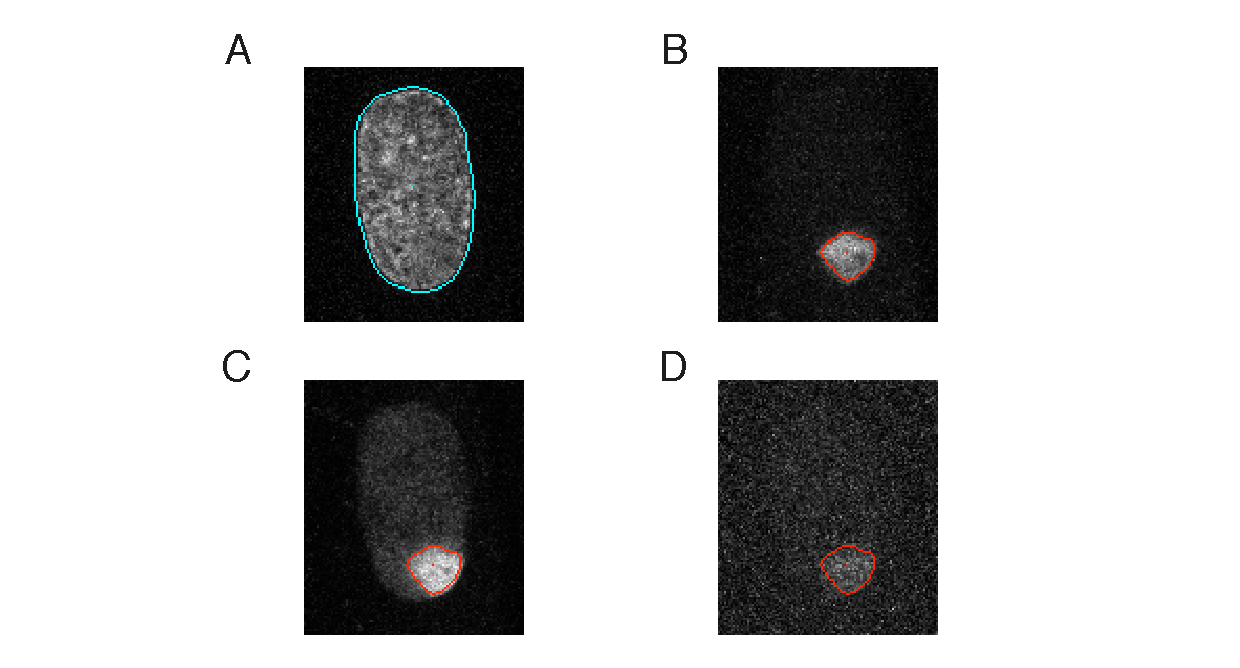
\includegraphics[width=1\textwidth]{Abbildungen/figure4_1.pdf}
		\caption{\textbf{3D fluorescence microscopy imaging of NER factor co-expression.} A) DAPI-stained DNA content measured in human primary fibroblast (Life technologies). DAPI segmentation at 461 nm  (green contour line) determines nuclear dimension. B-C) Nuclear expression of indirectly immuno-stained repair factors at 488 nm (B) and at 647 nm (C). Signals are quantified according to the nuclear contour (cyan contour line) segmented from the DAPI signal. D) DNA locally damaged by UV-irradiation and subsequently incubated for 60 minutes in the presence of 10 \textmu M EdU. Segmentation of the EdU signal is indicated by the red contour line.  (Experiments by P. Verbruggen)}
		\label{fig:coStaining}
	\end{center}
\end{figure}

To test whether the antibody co-staining experiment is suitable for the cross-correlation analysis, we measured XPC expression with a directly labelled antibody together with an indirect immuno-staining and correlated both signals. Fitting an error ellipse to these data (\textit{cf.}\ Figure \ref{fig:coExpressionData}A), as described in section  \ref{subsec:AccuFlipExp}, we estimated a relative measurement error of antibody labelling of 13\%, showing that the technique is sufficiently accurate to exploit the natural variability in protein expression for the cross-correlation analysis.
\begin{figure}[htbp]
	\begin{center}
		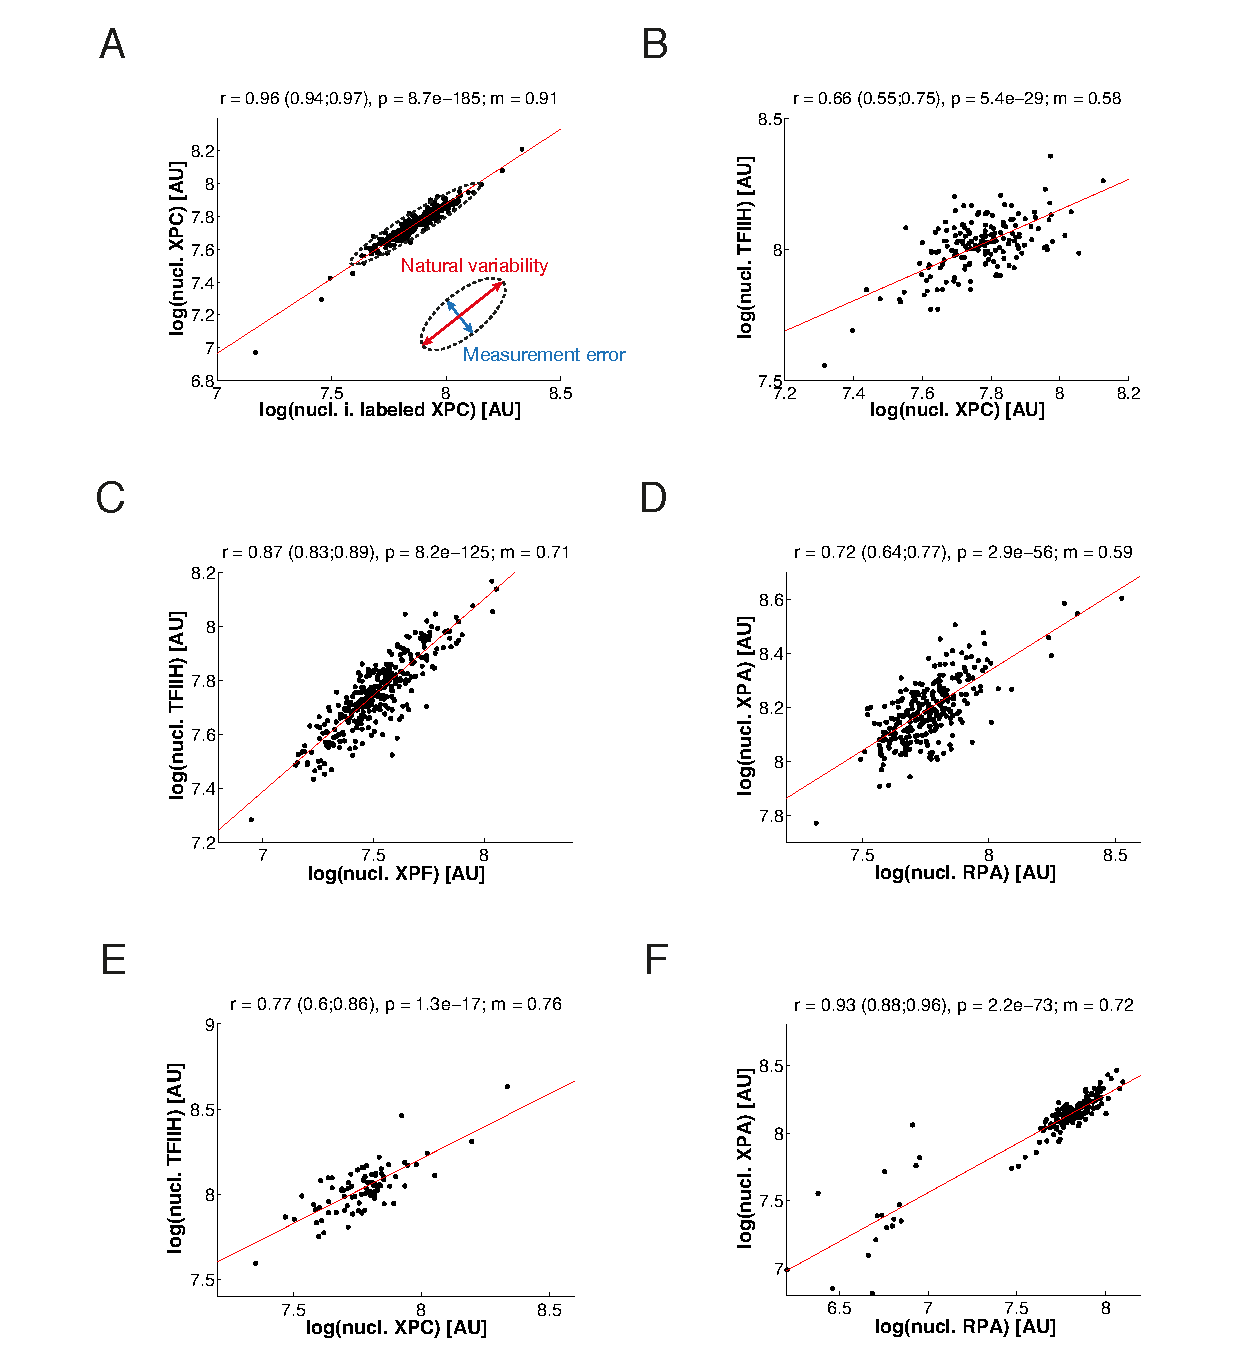
\includegraphics[width=1\textwidth]{Abbildungen/figureTAC_2.pdf}
		\caption{\textbf{NER factor cross-correlation is repair independent.} A) Scatter plot of indirectly antibody-stained XPC against a directly labelled antibody recognising XPC (n=336) as determined by quantitative (immuno) fluorescence microscopy. B-D) Pairwise correlations of indirectly antibody-labelled TFIIH against XPC (n=220, B), TFIIH against XPF (n=410, C) and XPA against RPA (n=350, D) in locally damaged cells. Expression values represent fluorescence intensities originating from the nucleus including the damaged region (signal quantification was performed analogous to \cite{Luijsterburg2010}). E-F) Scatter plots of the nuclear expression of TFIIH vs.\ XPC (n=85, E) and XPA vs.\ RPA (n=170, F) in undamaged cells. A-F) Red lines represent linear regression with correlation coefficient r, p-value and slope m. 95\% confidence bounds of all correlation coefficients r were estimated by non-parametric bootstrap and are given in brackets. (Experiments by P. Verbruggen)}
		\label{fig:coExpressionData}
	\end{center}
\end{figure}

\noindent As it turns out, all pairwise correlations of the measured co-staining experiments (\textit{cf.}\ Table \ref{tab:co-staining}) are strongly positive with correlation coefficients between 0.66 and 0.87 (\textit{cf.}\ Figure \ref{fig:coExpressionData}B-D and Figure \ref{fig:nuklearCrosscorrelation}). Notably, the result is irrespective of whether the acquired fluorescence signal is taken from the whole nucleus including the locally damaged area or only from the undamaged chromatin region (\textit{cf.}\ Figure \ref{fig:coExpressionData}B-D and \ref{fig:coExpressionData}E-F). This suggests that a dominating part of the positive correlation of nuclear NER factors is independent of the ongoing repair. As a consequence, we suspect that the regulatory mechanism determining the protein concentrations lies on a preceding level such as transcription or translation.\\  


%\begin{figure}[htbp]
%	\begin{center}
%		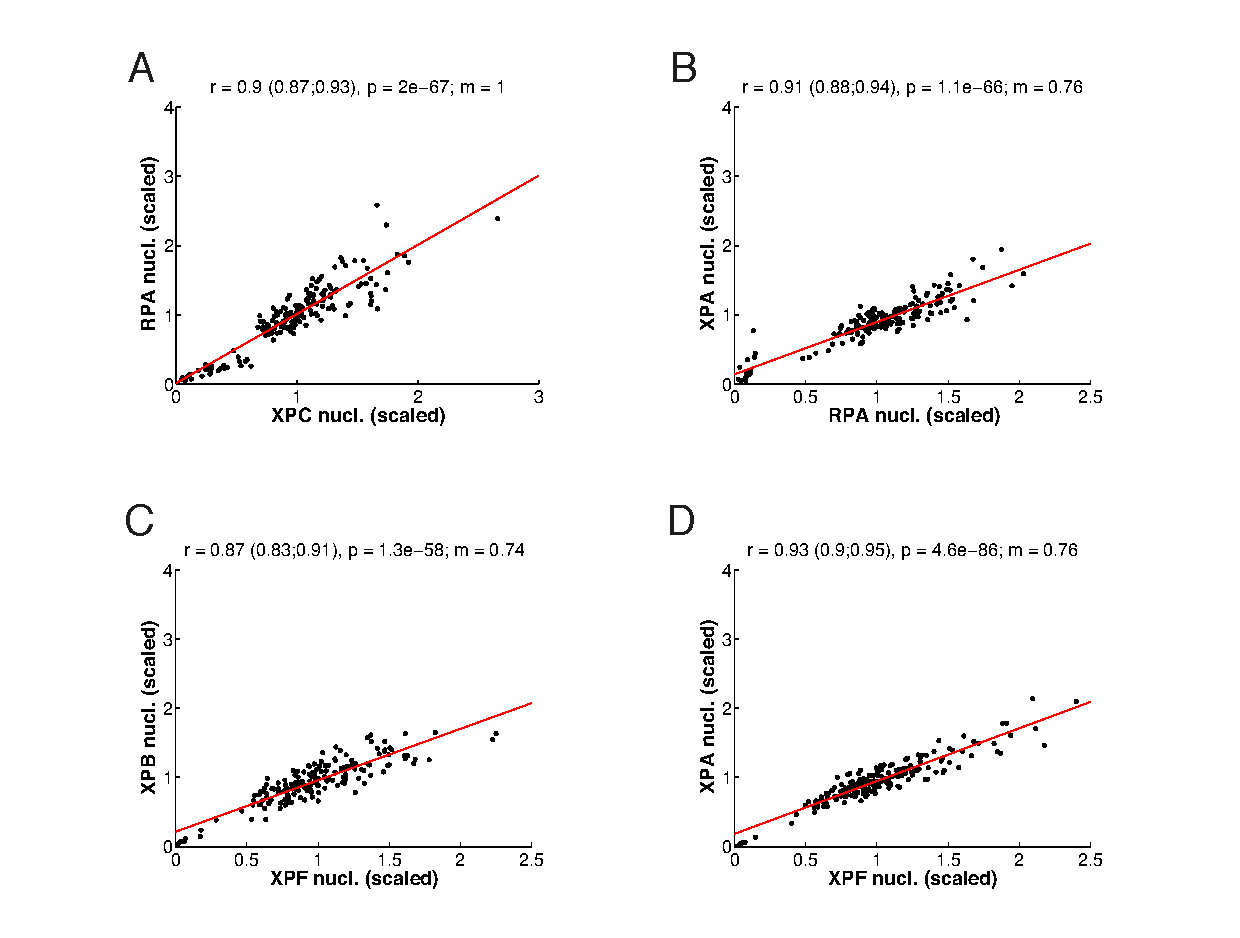
\includegraphics[width=1\textwidth]{Abbildungen/figure4_3.pdf}
%		\caption{\textbf{Blubb.} A) B) }
%		\label{fig:coExpressionData_woDamage}
%	\end{center}
%\end{figure}

\section {Cell cycle independent cross-correlation of NER factor expression}

To confirm the microscopy results we repeated the experiment by flow cytometry, this time, investigating the NER-factor expression in human brain pericytes. We established a double-staining protocol for XPA and RPA and observed that in this cell type the expression of the two repair factors also strongly correlates (\textit{cf.}\ Figure \ref{fig:FC_correlation}A and B).    
\begin{figure}[t]
	\begin{center}
		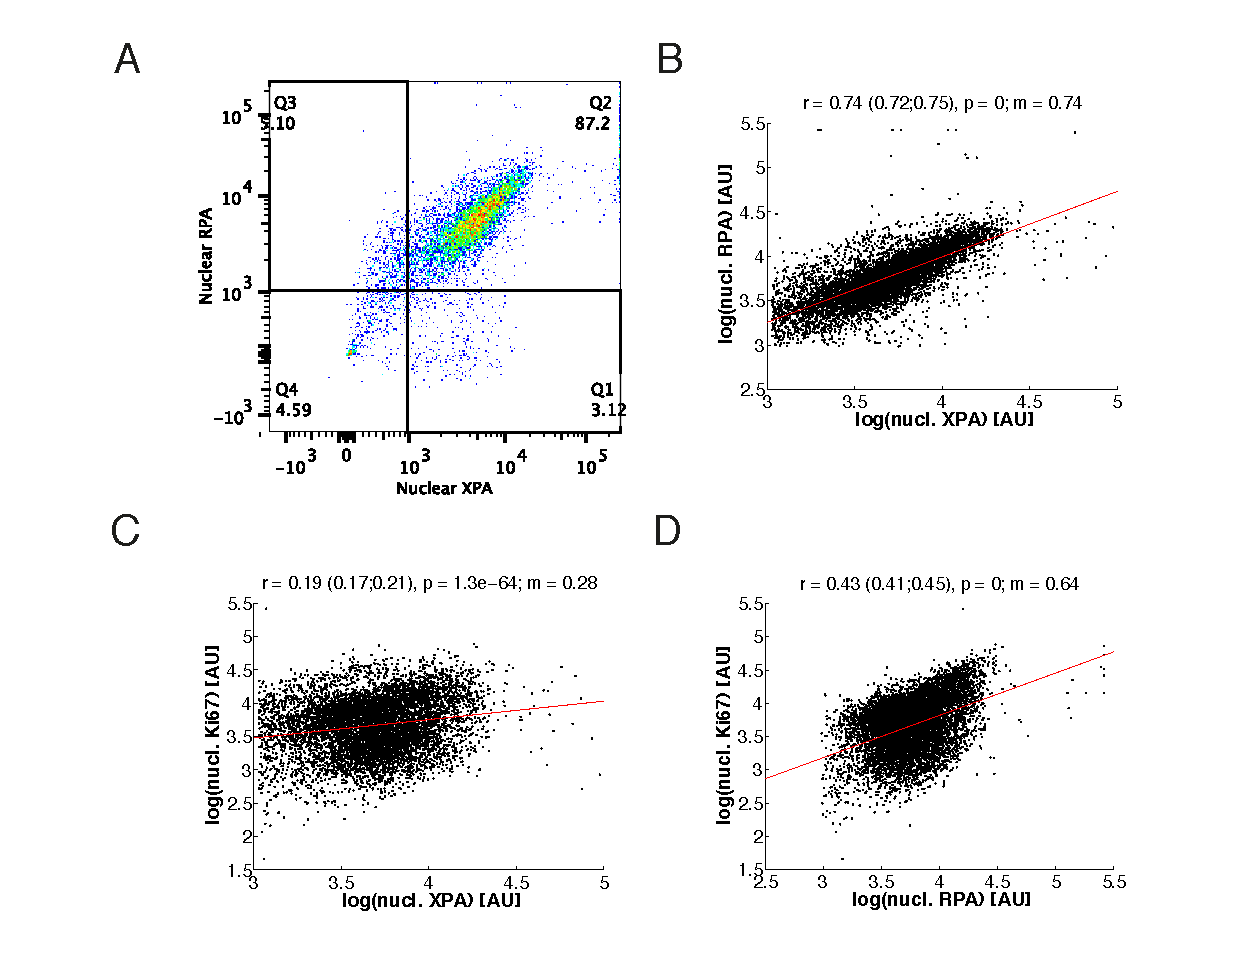
\includegraphics[width=1\textwidth]{Abbildungen/figureTAC_3.pdf}
		\caption{\textbf{Correlated expression of RPA and XPA in human brain pericytes.} A) Selection of XPA and RPA positive human brain pericytes (Q2) as determined by flow cytometry (n=8084). B-D) Nuclear expression of indirectly antibody-labelled RPA against XPA (B), Ki67 against XPA (C) and Ki67 against RPA (D). B-D) Red lines represent linear regression with correlation coefficient r, p-value and slope m. 95\% confidence bounds of all correlation coeffiecients r were estimated by non-parametric bootstrap and are given in brackets. (Experiments were performed in collaboration with M. Teichert)}
		\label{fig:FC_correlation}
	\end{center}
\end{figure}
Quantitatively, the correlation coefficients of the double-staining signals in both cell types (human brain pericytes and human primary fibroblasts) have the same order of magnitude. In particular, each value falls into the confidence interval of the other (\textit{cf.}\ Figure \ref{fig:FC_correlation}B and Figure \ref{fig:coExpressionData}D). To test whether this correlation is specific for proteins involved in DNA repair we measured the expression of the proliferation marker Ki67. Surprisingly, although the correlation between both repair factors and Ki67 is visibly reduced (XPA vs. Ki67 = 0.19 and RPA vs. Ki67 = 0.43 against XPA-RPA = 0.74), it is still significantly positively correlated (\textit{cf.}\ Figure \ref{fig:FC_correlation}C and D).\\
As Ki67 increases during cell cycle we asked, to what extent the observed protein correlation of Ki67 and the NER factors is cell-cycle dependent. To answer this question, we stained the cell's DNA using FxCycle violet and gated them according to their DNA content (\textit{cf.}\ Figure \ref{fig:FC_cell_cycle}A). Two distinct peaks denote the portion of cells traversing the G1 or the S and G2 phase, respectively. By sorting the protein expression values in accordance with their cell cycle phase we identified for each protein combination two contiguous regions revealing a general trend of increased protein expression during the S and G2 phase in comparison to the G1 phase (\textit{cf.}\ Figure \ref{fig:FC_cell_cycle}B-D).\\
Remarkably, whereas the correlation coefficients between XPA and RPA remain constant in both regimes (G1: 0.71, S+G2: 0.68, all: 0.74) the correlation between XPA and Ki67 disappears (G1: -0.072, S+G2: -0.068). Between RPA and Ki67 there is close to no correlation in the G1 phase but a significant small positive correlation in the S and G2 phase (G1: 0.12, S+G2: 0.29). These results strengthen the conclusions derived from the cross-correlation analysis in fibroblasts that NER factor expression is functionally co-regulated. In particular, the missing correlation between the nuclear factors and the cell-cycle marker after taking the cell-cycle into account suggests that the measured correlation is specific to NER proteins. 




%sentence about RPA - Ki67 correlation

\section{Measured average response agrees with model prediction}
To determine potential mutual dependencies in NER factor expression we performed two independent cross-correlation experiments, firstly based on microscopy of human fibroblast and secondly using flow cytometry in human brain pericytes. For both approaches we found conclusive evidence for a positive pairwise correlation of the nuclear repair factor concentration. As described in Section \ref{sec:crossCorelResponse} the measured cross-dependencies represent the entries of matrix $B$ in Eqn.\ \ref{eqn:matrixNotation}. In theory, the product of the inverse of $B$ and $A$ defines the vector of response coefficients. However, due to the strong multicolinearity the matrix $B$ has variance inflation factors (VIFs)\label{sec:vif} between 2.5 and 10.8 indicating that the variation of each protein is largely explained by a linear combination of the other protein expression values. VIFs measure how much of the predicted standard error of the response coefficient estimates is caused by the colinearity \cite{allison1999multiple}. For instance, for a VIF of 5 the estimated error is  about $\sqrt{5} \cong 2.3$ times as large as it would be if the variables in matrix $B$ were uncorrelated. 
\begin{figure}[t]
	\begin{center}
		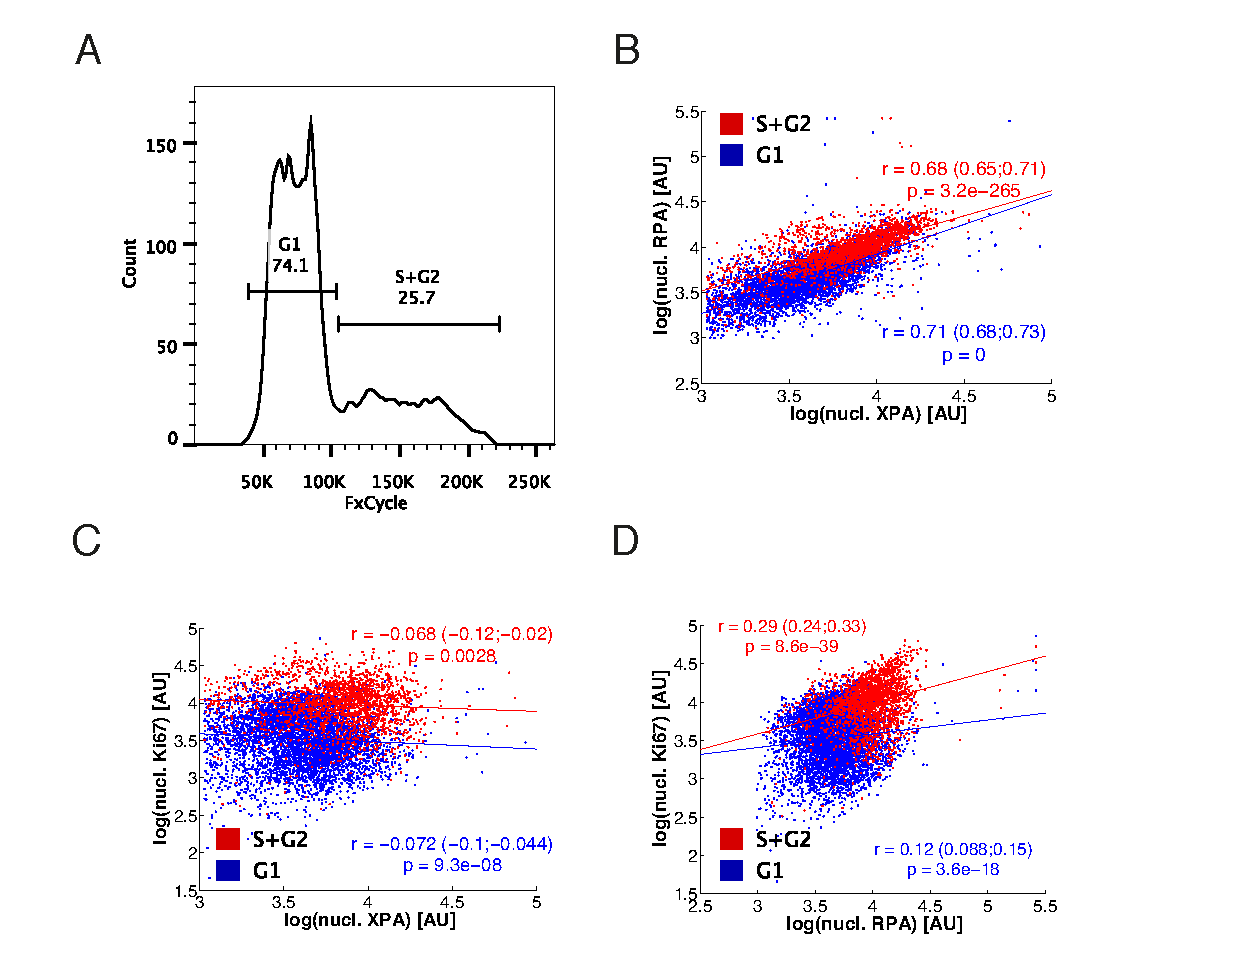
\includegraphics[width=1\textwidth]{Abbildungen/figureTAC_4.pdf}
		\caption{\textbf{NER factor cross-correlation is robust against cell cycle progression.} A) Distribution of fluorescently labelled DNA is proportional to the DNA content. Horizontal bars indicate the fractions of cells assigned to be in cell-cycle phase G1 (left peak, n=5469) and S+G2 (right peak, n=1945).  B-D) Individual regression analysis of the nuclear expression values sorted according to the corresponding cell-cycle phase (G1 in blue; S+G2 in red) for RPA vs. XPA (B), Ki67 vs. XPA (C) and Ki67 vs. RPA (D). B-D) Red and blue lines represent linear regression with correlation coefficient r and p-value. 95\% confidence bounds of all correlation coefficients r were estimated by non-parametric bootstrap and are given in brackets. (Experiments were performed in collaboration with M. Teichert)}
		\label{fig:FC_cell_cycle}
	\end{center}
\end{figure}  
Hence, we are not able to derive a reliable result for each response coefficient. However, it is possible to make an estimation of the average size of $\tilde{R}$. Consider $\nu$ as a function of the concentration of the repair factors $C_i$ for $i=1,\ldots,N$ multiplied with the initial amount of DNA lesions $L$:
\begin{equation}
	\nu = Lf(C_1,\ldots,C_N).
\end{equation}
Using, once more, the standard law for the propagation of uncertainty analogue to Eqn.\ \ref{eqn:lawoferrorPropagation}
 \begin{equation}
 \sigma(\nu) = \sqrt{\sum_{i=1}^{N}\left[\left(\frac{\partial \nu}{\partial C_i}\sigma(C_i) \right)^2 + \left(\frac{\partial \nu}{\partial L}\sigma(L)\right)^2 + \mathop{\sum_{j=1}^{N}}_{j\neq i}\left(\frac{\partial \nu}{\partial C_i} \frac{\partial \nu}{\partial C_i}\textrm{cov}(C_i,C_j)\right)^2\right]}
 \end{equation}  
 
and introducing the response coefficients from Eqn.\ \ref{eqn:responseCoefficientsII} we derive

\begin{equation}
	CV_{\nu}^2 = CV_{L}^2 + \sum_{i=1}^{N} \left((\tilde{R}_i\,CV_i)^2 + \mathop{\sum_{j = 1}^{N}}_{j\neq i} \tilde{R}_i\tilde{R}_j \frac{\textrm{cov}(C_i,C_j)}{\langle C_i \rangle\langle C_j\rangle}\right),
	\label{eqn:lawOfErrorPropII}
\end{equation}

where $\langle C_i \rangle$ denotes the mean repair factor concentration. With the simplifying assumption that $\tilde{R} = \tilde{R}_i$ for all $i = 1,\ldots,N$, which implies that all $\tilde{R_i}$ are the same, we can solve Eqn.\ \ref{eqn:lawOfErrorPropII} for $\tilde{R}$ and thereby derive an estimate for the average response coefficient:

\begin{equation}
	R = \sqrt{	\frac{CV_{\nu}^2 - CV_L^2}{\sum_{i=1}^{N} CV_i^2 + \mathop{\sum_{j=1}^{N}}_{j \neq i} \frac{\textrm{cov}(C_i,C_j)}{\langle C_i \rangle\langle C_j\rangle}}}.
	\label{eqn:averageResponse}
\end{equation} 


On the right-hand side we measured most of the $CV$s and about a third of the NER factor covariations (\textit{cf.}\ Table \ref{tab:proteinVariability}, Figure \ref{fig:coExpressionData} and \ref{fig:nuklearCrosscorrelation}). The missing entries were added by taking the average of the known elements. By inserting all measured and estimated quantities into Eqn.\ \ref{eqn:averageResponse} we calculated an average response coefficient of $\tilde{R} =$0.16. Remarkably, this result agrees exactly with the average response coefficients predicted by the model (\textit{cf.}\ Figure \ref{fig:controlCoefficients}) and thus, reconfirms the hypothesis of a small and collectively shared repair-rate control.     



%hier fehlt noch klarzumachen, dass cross-correlation einen positiven Beitrag zur Variabilität vieler Zellen untereinander hat aber in einer Zelle die Variabilität der Faktoren untereinenader geringer ist


